% Preamble
% ---
\documentclass{article}

% Packages
% ---
\usepackage{amsmath} % Advanced math typesetting
\usepackage[utf8]{inputenc} % Unicode support (Umlauts etc.)
\usepackage[english]{babel} % Change hyphenation rules
\usepackage{hyperref} % Add a link to your document
\usepackage{graphicx} % Add pictures to your document
\usepackage{listings} % Source code formatting and highlighting
\usepackage{amssymb} % Extra math symbols
\usepackage{algorithm}
\usepackage{algorithmic}
%\usepackage{float} % float images
% ---
\graphicspath{{./images/}}
%

\title{QR Decomposition Algorithms}
\author{Jaidon Lybbert, Fulin Li}
\date{\today{}}

\begin{document}

\maketitle{}
\tableofcontents{}
\listofalgorithms{}

\section{QR Decomposition}
\paragraph{}
The QR decomposition of an m-by-n matrix $A$ with $m>n$, is the matrix product $A = QR$, where $Q$ is an 
m-by-m unitary matrix, and $R$ is upper triangular \cite{bhaskar86qr}.

\subsection{Matrix Q}
\paragraph{}
The matrix $Q$ is a transformation which preserves inner products of column vectors of $R$. If the 
inner product space is real, the matrix $Q$ is equivalently orthogonal. One possibility of such a 
transformation is a rotation.
\paragraph{}
Another possibility of such an orthogonal transformation is a reflection. The matrix $Q$ in general 
is a combination of rotations and reflections.

\subsection{Matrix R}
\paragraph{}
The matrix $R$ is upper triangular, a form which has the following useful properties: (I) the determinant is equal to the product of the diagonal elements, (II) the eigenvalues are equal to the diagonal elements, (III) given the linear system $Rx = b$ it is easy to solve for $x$ by back substitution.

\section{Transformations}
\paragraph{}
In order to compute the decomposition of $A$, the matrix is iteratively transformed by unitary matrices $\{U_i : 0 < i < k\}$ until the product is upper triangular. This upper triangular matrix is the matrix $R$ in $A = QR$
\begin{equation}
	\label{eqn:r}
R = U_kU_{k-i} \dots U_1A.
\end{equation}
\paragraph{}
It follows, that the matrix $Q$ is composed of the set of inverse transformations
\begin{equation}
	\label{eqn:q}
Q = U_{1}^{T}U_{2}^{T} \dots U_{k}^{T}.
\end{equation}
\paragraph{}
The key to solving for $R$ is to choose transformations $U_i$ which produce zeros below the diagonal of the matrix product
\begin{equation}
	\label{eqn:update}
A^{(i)} = U_{i} \dots U_1A,
\end{equation}
and can iteratively be applied to achieve $R$. Two choices for $U_i$ are Householder reflections, and Givens rotations.

\subsection{Householder Reflections}
\paragraph{}
The Householder reflection is a unitary transformation represented by a matrix $H\in\mathbb{R}^{N\times{}N}$ which reflects a vector $\mathbf{u}\in\mathbb{R}^N$ across a hyperplane defined by its unit normal vector $\{\mathbf{w}\in\mathbb{R}^N: \|\mathbf{w}\|=1\}$. The transformation matrix is given by
\begin{equation}
	\label{eqn:Householder}
H = I - 2\mathbf{ww}^T
\end{equation}
where $I\in\mathbb{R}^{N\times{}N}$ is the identity matrix. \cite{bhaskar86householder} \cite{lambers21}

\begin{figure}[h]
\centering
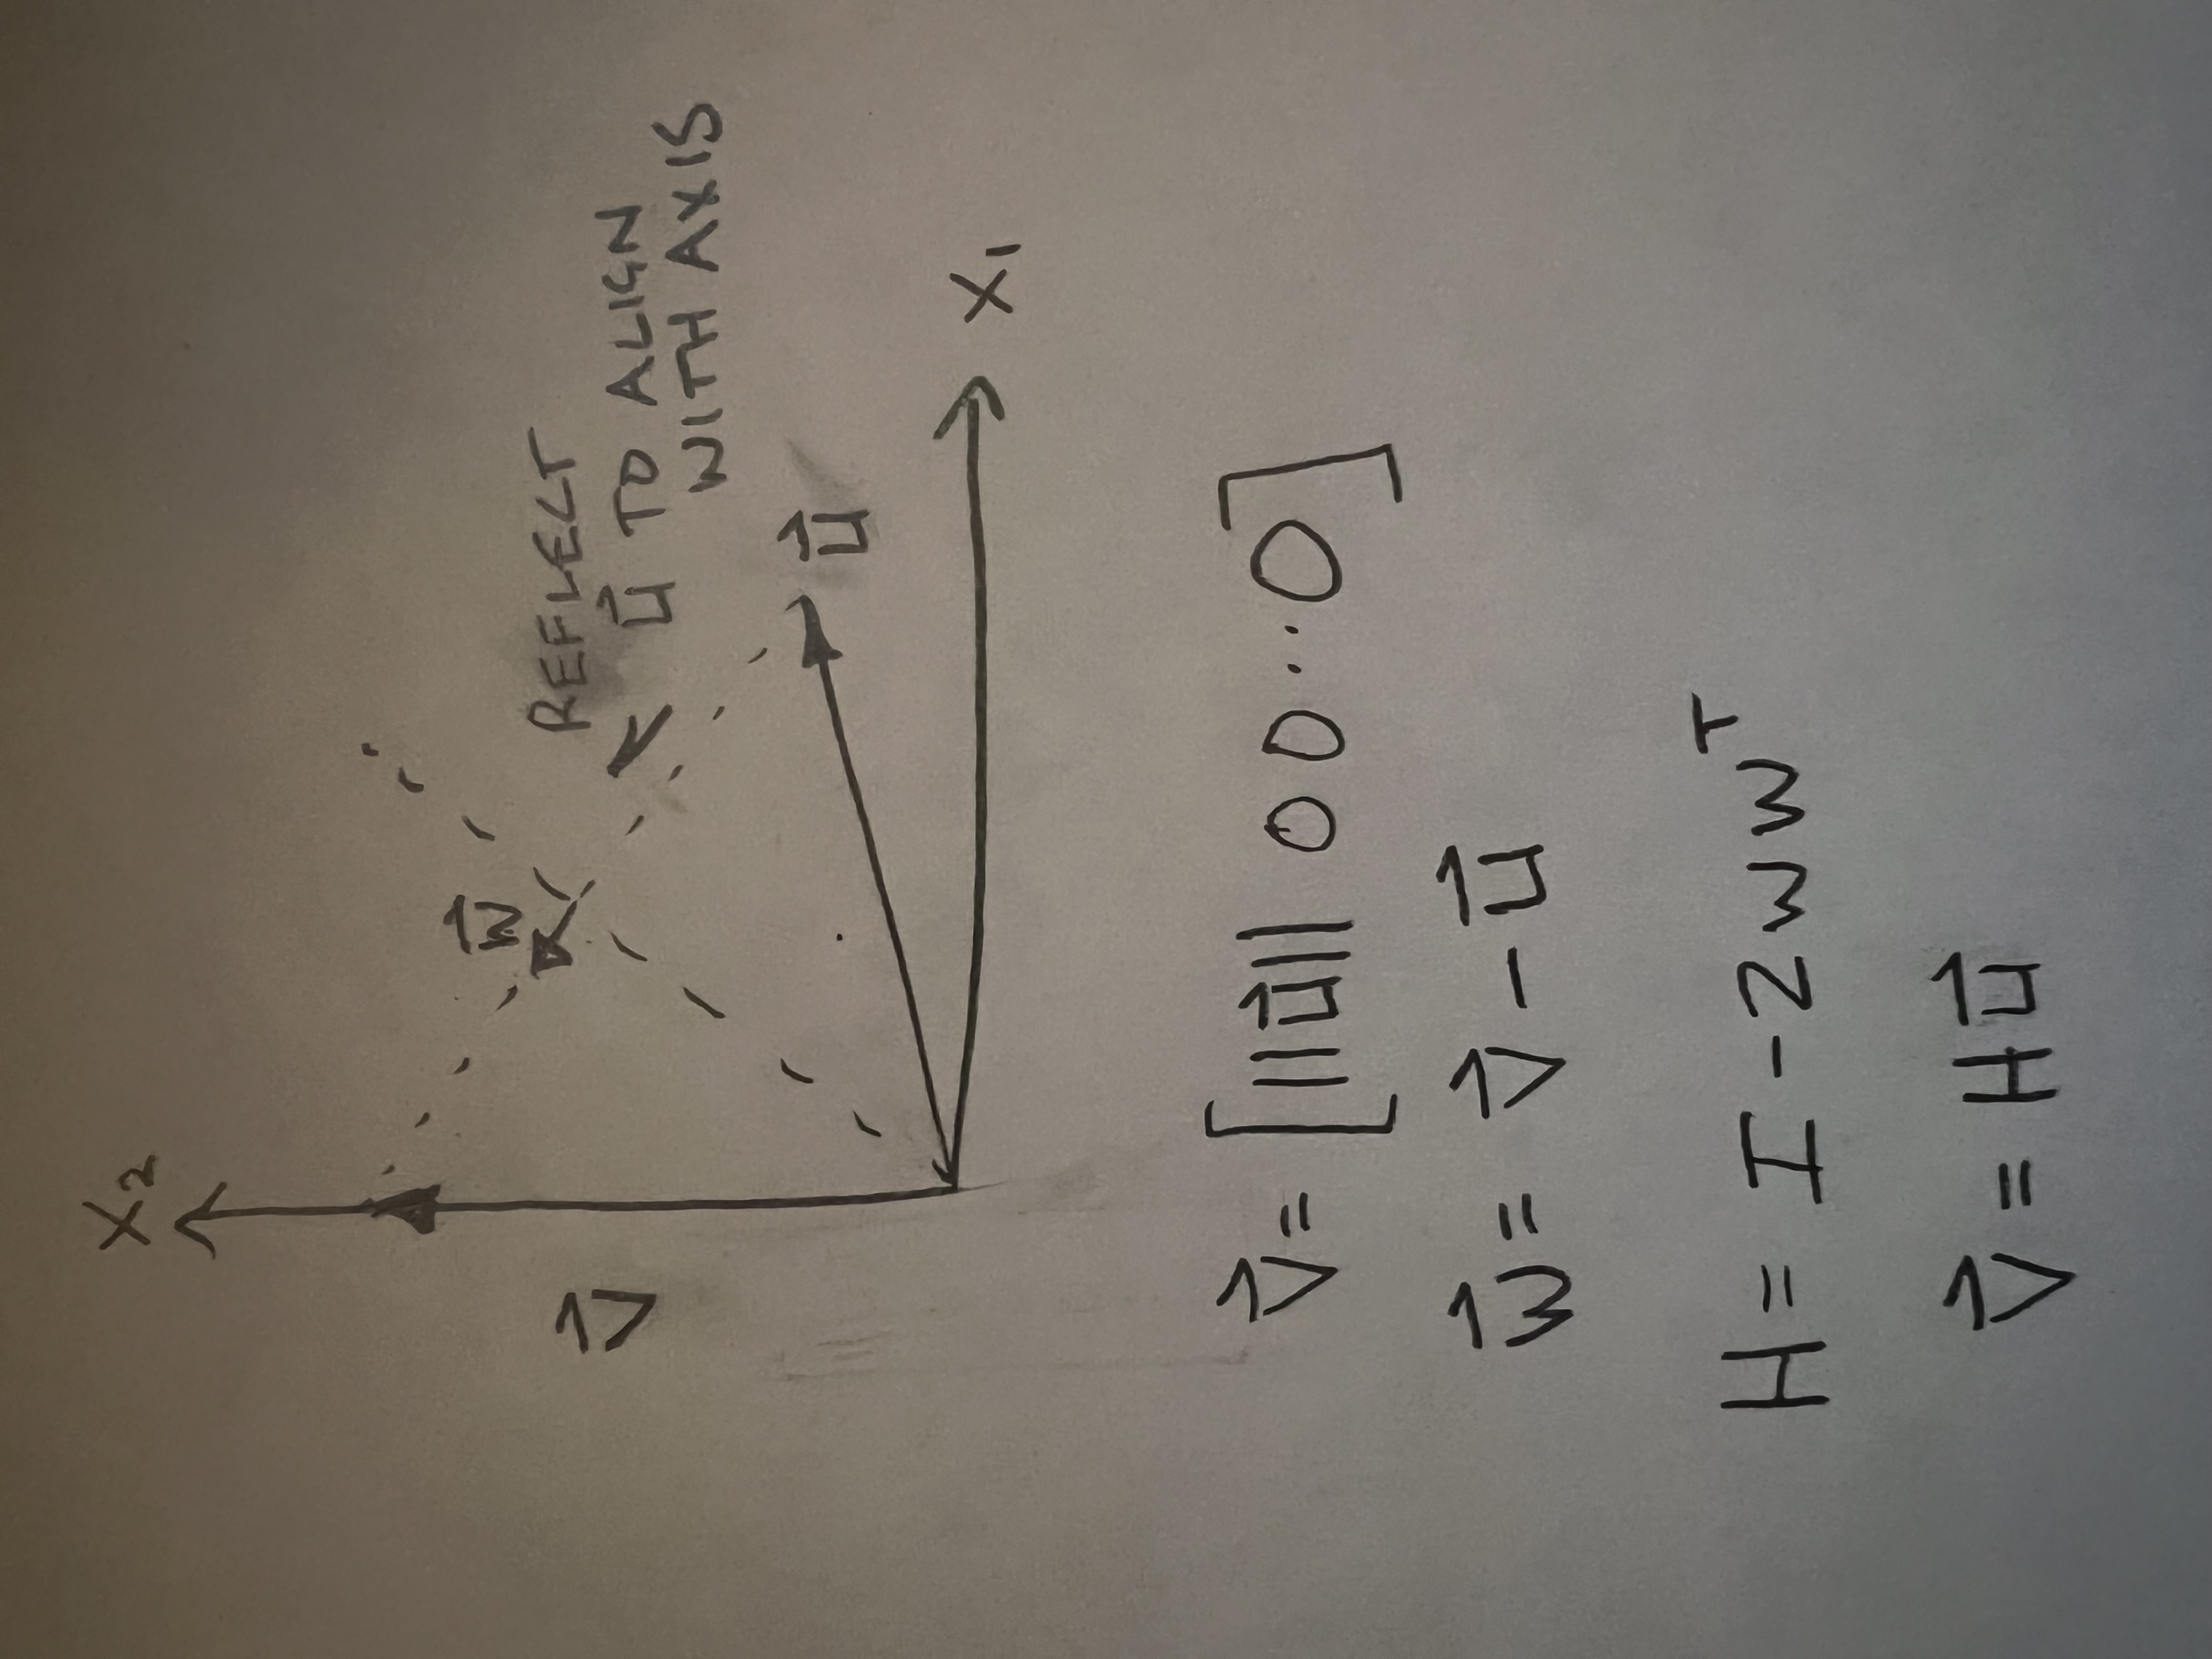
\includegraphics[width=75mm, angle=-90]{Householder2}
\caption{Geometric illustration of the reflection of a vector to an axis. The result of this transformation is that the vector now only has one non-zero component.}
\end{figure}

To reflect a vector $\mathbf{u}\in\mathbb{R}^N$ such that it points in the direction of a target vector $\mathbf{v}\in\mathbb{R}^N$, the transformation matrix $H$ can be computed by \eqref{eqn:Householder}, where $\mathbf{w}$ is given by

\begin{equation}
	\label{eqn:normal}
\mathbf{w} = \mathbf{v} - \mathbf{u},
\end{equation}

such that,

\begin{equation}
H\mathbf{u} = \|\mathbf{u}\|\mathbf{\hat{v}},
\end{equation}

where $\mathbf{\hat{v}}$ is a unit vector in the direction of the target vector $\mathbf{v}$.

\subsection{Givens Rotations}
\paragraph{}
A Givens rotation is a unitary transformation which rotates a vector $x$ counter-clockwise in a chosen plane. For example, possible Givens rotation matrices in $\mathbb{R}^4$ include
\begin{equation}
\begin{bmatrix}
1 & 0 & 0 & 0\\
0 & c & -s & 0\\
0 & s & c & 0\\
0 & 0 & 0 & 1
\end{bmatrix},
\begin{bmatrix}
c & -s & 0 & 0\\
s & c & 0 & 0\\
0 & 0 & 1 & 0\\
0 & 0 & 0 & 1
\end{bmatrix}, or
\begin{bmatrix}
1 & 0 & 0 & 0\\
0 & 1 & 0 & 0\\
0 & 0 & c & -s\\
0 & 0 & s & c
\end{bmatrix},
\end{equation}
where $c = \cos{\theta}$ and $s = \sin{\theta}$. Each of these examples have the effect of rotating the vector in different planes.

\paragraph{}
A Givens rotation can easily be computed to introduce zeros in the matrix $P$. The scalars $c$ and $s$ 
can be computed directly from elements in $P$ in order to zero out targeted elements\cite{golub} \cite{bhaskar86givens}. For 
example, say we want to zero out element $a_{21}$ in the matrix
\begin{equation}
P = 
\begin{bmatrix}
a_{11} & a_{12} & a_{13}\\
a_{21} & a_{22} & a_{23}\\
a_{31} & a_{32} & a_{33}
\end{bmatrix}.
\end{equation}
\paragraph{}
We target the second dimension of the column vector, so we rotate on the plane spanned by 
the first two dimensions. The Givens rotation to rotate 
on this plane is of the form
\begin{equation}
G = 
\begin{bmatrix}
c & -s & 0\\
s & c & 0\\
0 & 0 & 1
\end{bmatrix}
\end{equation}
which will leave the third row of $P$ unmodified. We are aligning the column vector with the axis of the first 
dimension, making the component of the vector along the second dimension zero. Fig. \ref{GivensFig} shows a geometric 
illustration of the rotation.

\begin{figure}
\centering
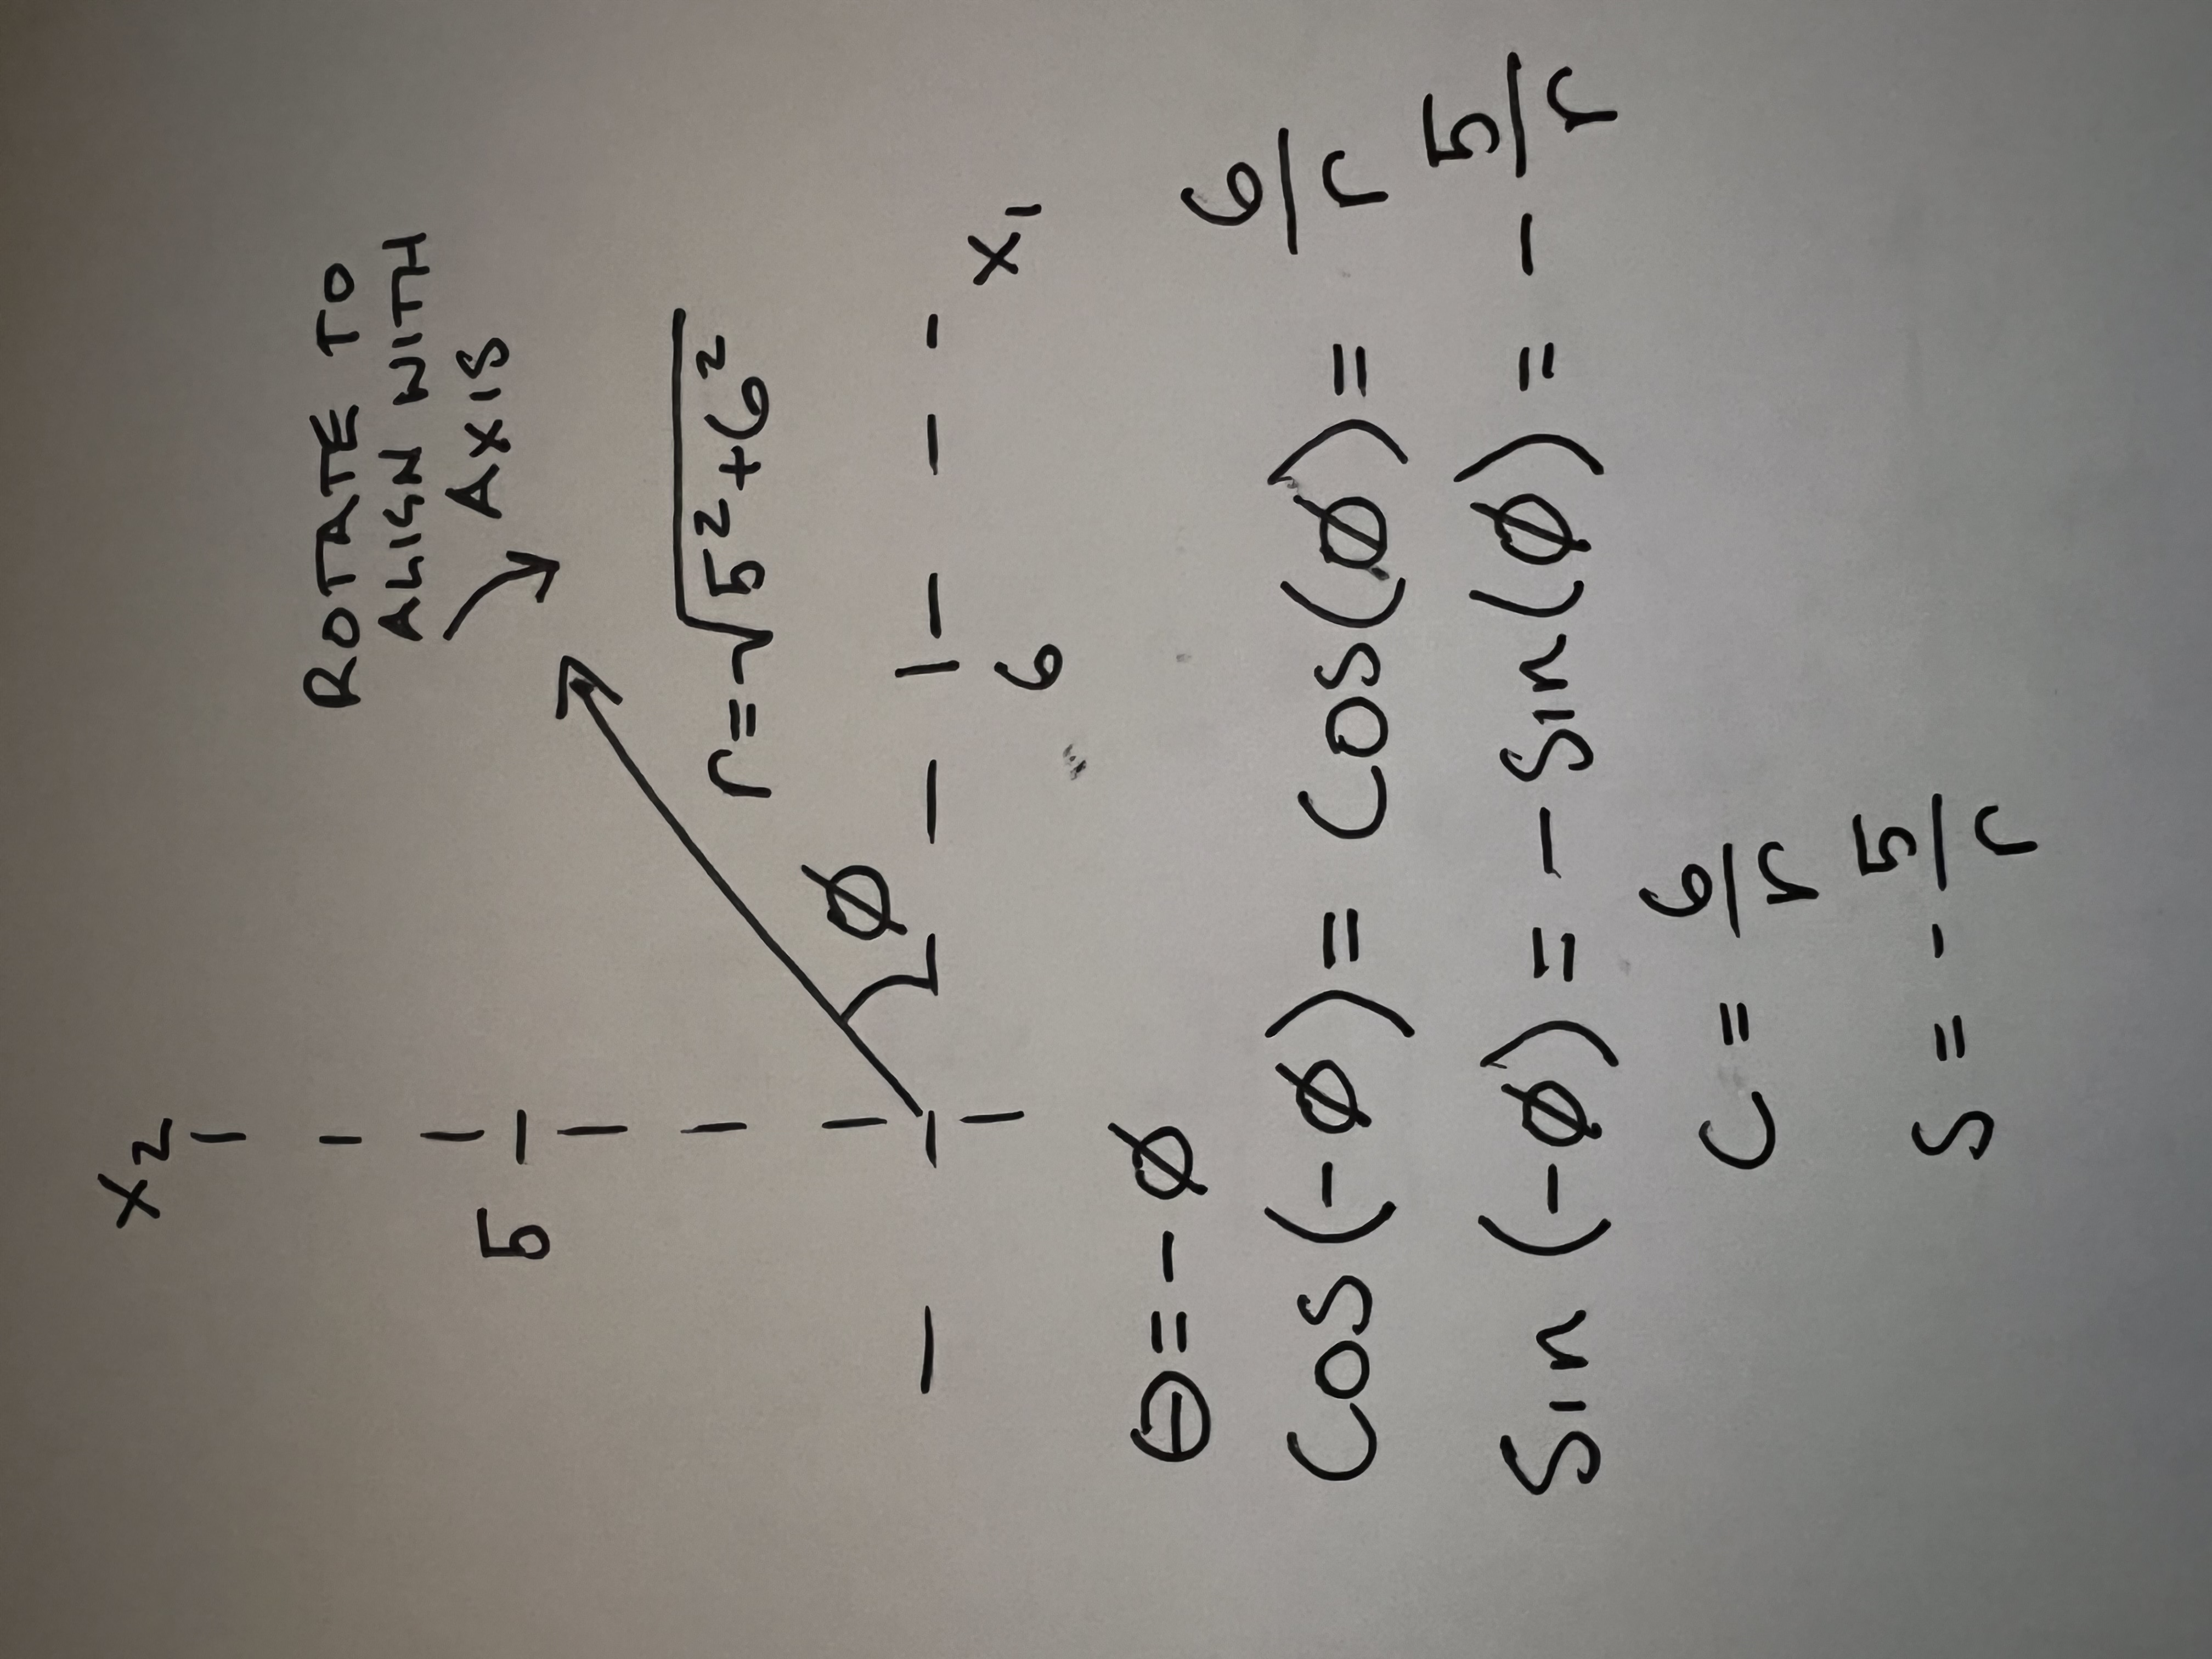
\includegraphics[width=75mm, angle=-90]{Givens1}
\caption{Geometric illustration of the rotation of a vector in $\mathbb{R}^3$ about the axis of basis vector ${x3}$ to align with the basis vector ${x1}$. The result of this transformation is that the component of the transformed vector in the direction of the basis vector $x2$ is zero, corresponding to a zero introduced in the transformed matrix.}
\label{GivensFig}
\end{figure}

\paragraph{}
The scalars $c$ and $s$ of matrix $G$ are computed directly from the values in matrix P by the equations 
\begin{equation}
c = \frac{a_{11}}{r}, 
\end{equation}
\begin{equation}
s = -\frac{a_{21}}{r}, 
\end{equation}
where
\begin{equation}
 r=\sqrt{a_{11}^2 + a_{21}^2}
\end{equation}
The transformation to introduce the zero is then
\begin{equation}
P = GP_{prior} =
\begin{bmatrix}
c & -s & 0\\
s & c & 0\\
0 & 0 & 1
\end{bmatrix}
\begin{bmatrix}
a_{11} & a_{12} & a_{13}\\
a_{21} & a_{22} & a_{23}\\
a_{31} & a_{32} & a_{33}
\end{bmatrix}
\end{equation}

\begin{equation}
P = GP_{prior} =
\begin{bmatrix}
a_{11}/r & a_{21}/r & 0\\
-a_{21}/r & a_{11}/r & 0\\
0 & 0 & 1
\end{bmatrix}
\begin{bmatrix}
a_{11} & a_{12} & a_{13}\\
a_{21} & a_{22} & a_{23}\\
a_{31} & a_{32} & a_{33}
\end{bmatrix}
\end{equation}

\begin{equation}
P = GP_{prior} =
\begin{bmatrix}
a_{11}/r & a_{21}/r & 0\\
-a_{21}/r & a_{11}/r & 0\\
0 & 0 & 1
\end{bmatrix}
\begin{bmatrix}
a_{11} & a_{12} & a_{13}\\
a_{21} & a_{22} & a_{23}\\
a_{31} & a_{32} & a_{33}
\end{bmatrix}
\end{equation}

\begin{equation}
P = 
\begin{bmatrix}
\frac{a_{11}a_{11} + a_{21}a_{21}}{r} & \frac{a_{11}a_{12} + a_{21}a_{22}}{r} & \frac{a_{11}a_{13} + a_{21}a_{23}}{r}\\
\frac{-a_{21}a_{11}+ a_{11}a_{21}}{r} & \frac{-a_{21}a_{12} + a_{11}a_{22}}{r} & \frac{-a_{21}a_{13} + a_{11}a{23}}{r} \\
a_{31} & a_{32} & a_{33}
\end{bmatrix}
\end{equation}

\begin{equation}
P = 
\begin{bmatrix}
\frac{a_{11}a_{11} + a_{21}a_{21}}{r} & \frac{a_{11}a_{12} + a_{21}a_{22}}{r} & \frac{a_{11}a_{13} + a_{21}a_{23}}{r}\\
0 & \frac{-a_{21}a_{12} + a_{11}a_{22}}{r} & \frac{-a_{21}a_{13} + a_{11}a{23}}{r} \\
a_{31} & a_{32} & a_{33}
\end{bmatrix}
\end{equation}
the zero is introduced in the desired location.



\section{Algorithms}
\subsection{Householder QR}
\paragraph{}
In order to get the upper triangular matrix $R \in\mathbb{R}^{N\times{}N}$ given a matrix $A \in\mathbb{R}^{M\times{}N}$ using householder reflections, we can use \eqref{eqn:r}, where the set of unitary transformations is a set of padded householder matrices $\{U_i\in\mathbb{R}^{M\times{}M} : 0 < i < N\}$, so that,
\begin{equation}
R = U_{N-1} U_{N-2} \dots U_1A.
\end{equation}

Let 
\begin{equation}
A^{(i)}=U_{i} \dots U_1A
\end{equation}
represent the i-th update of matrix A, so $A^{(N)}=R$ and $A^{(0)} = A$. Then the calculation of $U_i$ depends on the updated matrix $A^{(i-1)}$.
\paragraph{}
The householder QR algorithm procedure is to iteratively calculate each matrix $U_i$ from $A^{(i-1)}$, then update the matrix $A^{(i)} = U_iA^{(i-1)}$ for the next iteration, until $A^{(N)}=R$ is achieved. At each iteration, $U_i$ is determined such that the i-th column of $A^{(i-1)}$ is transformed so that all elements below the diagonal of the column are zero in the updated matrix $A^{(i)} = U_iA^{(i-1)}$ \cite{golub} \cite{doi:10.1137/19M1296367}.

For example,

\begin{equation}
A^{(1)} =
\begin{bmatrix}
\times & \times & \cdots & \times & \times\\
0 & \times  & \cdots & \times & \times\\
0 & \times  & \cdots & \times & \times\\
\vdots & \vdots  & \ddots & \vdots & \vdots\\
0 & \times  & \cdots & \times & \times\\
\end{bmatrix}
\end{equation}

\begin{equation}
A^{(2)} =
\begin{bmatrix}
\times & \times & \cdots & \times & \times\\
0 & \times  & \cdots & \times & \times\\
0 & 0 & \cdots & \times & \times\\
\vdots & \vdots  & \ddots & \vdots & \vdots\\
0 & 0  & \cdots & \times & \times\\
\end{bmatrix}
\end{equation}

\begin{equation}
A^{(N-1)} = R =
\begin{bmatrix}
\times & \times & \cdots & \times & \times\\
0 & \times  & \cdots & \times & \times\\
0 & 0 & \cdots & \times & \times\\
\vdots & \vdots  & \ddots & \vdots & \vdots\\
0 & 0  & \cdots & 0 & \times\\
\end{bmatrix}
\end{equation}

Each padded householder transformation matrix $U_{i}\in\mathbb{R}^{M\times{}M}$ is created by padding a householder matrix $H_{i}\in\mathbb{R}^{(M-i)\times{}(M-i)}$ with ones along the upper diagonal.

\begin{equation}
U_{i}\in\mathbb{R}^{M\times{}M} =
\begin{bmatrix}
1 & 0 & \cdots & 0  & 0\\
0 & 1  & \cdots & 0 & 0\\
0 & 0 & \cdots & 0 & 0\\
\vdots & \vdots  & \ddots & \vdots & \vdots\\
0 & 0  & \cdots & 0 & H_{i}\in\mathbb{R}^{(M-i)\times{}(M-i)}\\
\end{bmatrix}
\end{equation}

Let $A'^{(i)}\in\mathbb{R}^{(M-i)\times{}(M-i)}$ be the lower right submatrix of $A^{(i)}$, such that

\begin{equation}
A^{(i)} =
\begin{bmatrix}
1 & 0 & \cdots & 0  & 0\\
0 & 1  & \cdots & 0 & 0\\
0 & 0 & \cdots & 0 & 0\\
\vdots & \vdots  & \ddots & \vdots & \vdots\\
0 & 0  & \cdots & 0 & A'^{(i)}\in\mathbb{R}^{(M-i)\times{}(M-i)}\\
\end{bmatrix}
\end{equation}

Each householder matrix $H_{i}$ is calculated by obtaining $\mathbf{w}_i\in\mathbb{R}^{M-i}$ from the submatrix $A'^{(i-1)}\in\mathbb{R}^{(M-i+1)\times{}(M-i+1)}$, such that

\begin{equation}
A^{(i)} =
\begin{bmatrix}
1 & 0 & \cdots & 0  & 0\\
0 & 1  & \cdots & 0 & 0\\
0 & 0 & \cdots & 0 & 0\\
\vdots & \vdots  & \ddots & \vdots & \vdots\\
0 & 0  & \cdots & 0 & A'^{(i)}\in\mathbb{R}^{(M-i)\times{}(M-i)}\\
\end{bmatrix}
\end{equation}

and

\begin{equation}
A'^{(i)} =
\begin{bmatrix}
\mathbf{u_i} & \mathbf{c_2}  & \cdots & \mathbf{c_j} & \cdots \mathbf{c}_{M-1}\\
\end{bmatrix}.
\end{equation}
where $\mathbf{c}_j$ is the j-th column of $A'^{(i)}$, and $\mathbf{u}_i\in\mathbb{R}^{M-i}$ is used as the vector $\mathbf{u}$ in \eqref{eqn:normal} to calculate $\mathbf{w}_{i}$.
\paragraph{}
Let
\begin{equation}
\mathbf{v}_i\in\mathbb{R}^{M-i} = 
\begin{bmatrix}
\|\mathbf{u_i}\| \\
0  \\
\vdots \\
0 \\
\end{bmatrix}.
\end{equation}

then $\mathbf{w}_i$ is obtained from $\mathbf{u}_i$ and $\mathbf{v}_i$ according to \eqref{eqn:normal}, $H_i$ is determined by \eqref{eqn:Householder} from $\mathbf{w}_i$, $U_i$ is obtained by padding $H_i$, $A^{(i+1)}$ is obtained by \eqref{eqn:update}, and the iterations continue until R is achieved, as in \eqref{eqn:r}.

\paragraph{}
Q can easily be computed by keeping a running matrix product according to \eqref{eqn:q} during the iterations of the algorithm.

\paragraph{}
The Householder algorithm can be written concisely using the notation in \cite{}. For the matrix $A$, the notation $A_{k:m,k}$ is defined as the submatrix of A formed by the k-th through m-th rows of the k-th column. 


\begin{algorithm}
\caption{Calculate $A = QR$ using Householder reflections}
\label{alg1}
\begin{algorithmic}[1]
\FOR{$k=1$ to $n$}
\STATE{$u = A_{k:m,k}$}
\STATE{$v_k = sign(u_1)\|u\|_{2}e_{1}+u$}
\STATE{$v_k = v_k/\|v_{k}\|_{2}$}
\STATE{$A_{k:m,k:n} = A_{k:m,k:n}-2v_{k}(v_{k}^{T}A_{k:m,k:n})$}
\ENDFOR
\end{algorithmic}
\end{algorithm}
In Algorithm~\ref{alg1}, the householder vector $\mathbf{w}$ overwrites the vector $\mathbf{v}$. Recall, $U=H$ in \eqref{eqn:r} for the Householder QR algorithm. The transformation of $A$ by the orthogonal Householder matrix $U$ in \eqref{eqn:r} is implicit in the last line of the for loop, where $A$ is distributed through \eqref{eqn:Householder}.

\subsubsection{FLOPS}
\paragraph{}
We count the average FLOPS in \ref{alg1} line-by-line in the inner loop, and multiply by N columns of the outer loop.

\textbf{Line 2}
The copy operation is realized by a for-loop iterating over the copied column. On average, the length of this column is $m/2$, so the contribution is $N * M / 2$ FLOPs.

\textbf{Line 3}
The calculation of the magnitude of vector u takes an average M / 2 FLOPs, which is added to an additional M FLOPs for the multiply-accumulate into $v_k$ for a total contribution of $3 * N * M / 2$ FLOPs.

\textbf{Line 4}
Again, the magnitude of vector $v_k$ requires an average M / 2 FLOPs, and the division adds another M / 2 FLOPs. The total contribution is $N * M$ FLOPs.

\textbf{Line 5}
The vector matrix product $(v_{k}^{T}A_{k:m,k:n})$ consists of a vector matrix product contributing $$\frac{1}{N} \sum_{k=0}^N (M-k)(N-k)$$ FLOPs on average. The following vector-vector product $v_{k}(v_{k}^{T}A_{k:m,k:n})$ contributes the same number of FLOPs.

\subsubsection{Parallelism}
\paragraph{}
The dependence of $U_i$ on $A^{(i-1)}$ limits the parallelism of the Householder QR algorithm, such that the outer loop of Algorithm~\ref{alg1} can't be parallelized, and we must repeat lines 2-5, for each of N columns.

The matrix update portion $A_{k:m,k:n} = A_{k:m,k:n}-2v_{k}(v_{k}^{T}A_{k:m,k:n})$ can be computed by parallel matrix multiply algorithms, however these operations are interspersed with the computation of the padded householder matrix $U_i$, which is highly sequential. If the parallel portions of this algorithm are implemented on a GPU, and the sequential portions on the host CPU, memory bandwidth and latency become a significant speed and efficiency bottleneck, as the data is passed back and forth between CPU memory and GPU memory \cite{doi:10.1137/19M1296367} \cite{BISCHOFC1987TWrf}.

\subsection{WY-representation}

For the factored form of $Q \in \mathbb{R}^{M \times M} = {Q_1}{Q_2}{\dots}{Q_j}{\dots}{Q_n}$ where $Q_j = {I_m} - {\beta{}_j}{\mathbf{w}_j}{\mathbf{w}_j}^T$ and the factors ${\mathbf{w}_j}$, ${\beta{}_j}$ are stored as  

\begin{equation}
V \in \mathbb{R}^{M \times n} =
\begin{bmatrix}
\mathbf{w}_1 & \mathbf{w}_2 & \cdots & \mathbf{w}_j & \cdots & \mathbf{w}_{n}
\end{bmatrix}
\end{equation}

\begin{equation}
B \in \mathbb{R}^{n} = 
\begin{bmatrix}
\beta{}_1 & \beta{}_2 & \cdots & \beta{}_{j} & \cdots & \beta{}_{n}
\end{bmatrix}
\end{equation}

 the W and Y factors such that $Q = I_m - {W}{Y}^T$ can be calculated from $V$, and $B$ \cite{golub} \cite{doi:10.1137/19M1296367}. See Algorithm \ref{wy}.

\begin{algorithm}
\caption{Calculate W, Y from the factored form of Q: $V$ and $B$}
\label{wy}
\begin{algorithmic}[1]
\STATE{$Y = \mathbf{w}_{1}$}
\STATE{$W = \beta_{1}\mathbf{w}_{1}$}
\FOR{$j=2$ to $r$}
\STATE{$z = \beta_j(I_m-WY^T)\mathbf{w}_{j}$}
\STATE{$W = [W|z]$}
\STATE{$Y = [Y|\mathbf{w}_{j}]$}
\ENDFOR
\end{algorithmic}
\end{algorithm}



\subsection{Block QR}
\paragraph{}
 The Block QR algorithm reduces the memory workload by combining multiple householder transformations into a single matrix via the WY-representation of matrix products, before doing the matrix update \cite{BISCHOFC1987TWrf}.

\paragraph{}
Returning to equation \eqref{eqn:r}, the Block QR algorithm splits the matrix $A \in\mathbb{R}^{M\times{}N}$ into $b = ceil(\frac{N}{n_b})$ panels $\{P_j \in \mathbb{R}^{M\times{}n_b} : 0 < j <= b\}$ of width $n_b$ \cite{doi:10.1137/19M1296367}.

\begin{equation}
A = 
\begin{bmatrix}
P_1 & P_2 & \cdots & P_b
\end{bmatrix}
\end{equation}

For each panel, $n_b$ householder vectors $\{\mathbf{w}_k \in \mathbb{R}^M : 0 < k <= n_b\}$ are determined by performing the Householder QR decomposition on the panel, and saving the vectors $\mathbf{w}_k$ at each iteration to form a transformation $U_j \in \mathbb{R}^{M\times M} = I - W_jY_j^T$ using the WY transformation, such that the set $\{U_j : 0 < j <= b\}$ satisfies \eqref{eqn:r}.

$W_j$ and $Y_j$ are computed using the Householder factors $\mathbf{w}_k$ and $\beta{}$ in the general householder equation $H = I - \beta{}\mathbf{w}\mathbf{w}^T$, where in our case $\beta = 2$ as in \eqref{eqn:Householder}.

\begin{equation}
W_j, Y_j = wy\_representation(V_j, B_j)
\end{equation}

where 
\begin{equation}
V_j \in \mathbb{R}^{M \times n_b} =
\begin{bmatrix}
\mathbf{w}_1 & \mathbf{w}_2 & \cdots & \mathbf{w}_{n_b}
\end{bmatrix}
\end{equation}
and
\begin{equation}
B_j \in \mathbb{R}^{n_b} = 
\begin{bmatrix}
\beta{}_1 & \beta{}_2 & \cdots & \beta{}_{n_b}
\end{bmatrix}
\end{equation}

At each iteration $j$ of the block QR algorithm, $U_j$ is computed by the W-Y representation, then the sub-matrix $A'^{(j)} \in \mathbb{R}^{(m - (j * n_b)) \times (n - (j * n_b))}$ is updated by $A'^{(j)} = U_{j}A'^{(j-1)}$ \cite{doi:10.1137/19M1296367} \cite{golub}.

\paragraph{}
When $j = b$ then $(j * n_b) = N$, the width of sub-matrix $A'^{(j)}$ is zero, the matrix $A^{(j)} = A^{(n_b)} = R$, and the decomposition is complete.

\paragraph{}
Using the same notation as in Algorithm \ref{alg1}, the Block Householder QR algorithm can be written concisely as
\begin{algorithm}
\label{blockqr}
\caption{Block Householder QR Decomposition}
\begin{algorithmic}[1]
\STATE{$Q=I_m$}
\STATE{$\lambda = 1$}
\STATE{$k = 0$}
\WHILE{$\lambda \leq n$}
\STATE{$\tau \leftarrow min(\lambda + r - 1, n)$}
\STATE{$k = k + 1$}
\STATE{$A_{\lambda:m,\lambda:\tau} \leftarrow Householder\_qr(A_{\lambda:m,\lambda:\tau})$}
\STATE{$W_k, Y_k \leftarrow WY\_transform(V_k)$}
\STATE{$A_{\lambda:m, \tau + 1:n} = (I - W_{k}Y_{k}^T)^TA_{\lambda:m, \tau + 1:n}$}
\STATE{$Q_{:,\lambda:m} = Q_{:,\lambda:m}(I - W_{k}Y_{k}^T)$}
\STATE{$\lambda = \tau + 1$}

\ENDWHILE
\end{algorithmic}
\end{algorithm}

\bibliographystyle{plain}
\bibliography{refs}

\end{document}